\chapter{Gaussian Mixture Models}
\label{ch:gmm}

In \chapterref{speaker-recognition-system} was discussed the use of a model $\lambda_j$ for each enrolled speaker to be identified, and models $\lambda_{hyp}$ and $\lambda_{bkg}$ for a claimed speaker and for the background composed of all enrolled speakers, respectively, to perform a verification process. As the features from the speech signal (discussed in \chapterref{feature-extraction}) have unknown values until the moment of extraction, it is reasonable to model the ASR to accept random values.

For all sorts of probability distributions, the Gaussian (or normal) is the one that best describes the behavior of a random variable of unknown distribution, due to the central limit theorem. Its equation for a D-dimensional space is

\begin{equation}
    \pdf{\dvec{x}} = p(\dvec{x},\dvec{\mu},\dvec{\Sigma}) = \dgaussian{x}{\mu}{\Sigma},
    \label{eq:gaussian}
\end{equation}

\noindent where $\dvec{x}$ is a $D$-dimensional input vector, $\dvec{\mu}$ is the $D$-dimensional vector of means and $\dvec{\Sigma}$ is the $D \times D$ matrix of covariances. The vector $(\dvec{x} - \dvec{\mu})'$ is the transposed of the colum-matrix $(\dvec{x} - \dvec{\mu})$.

For the speaker recognition, a weighted sum of $p_i(\dvec{x})$ is used to model the system, trying to estimate the composition that best represents the training data. This weighted sum is named Gaussian Mixture Model (GMM), \refbib{Reynolds}{reynolds.1992}, and is given by

\begin{equation}
    \postpdf{\dvec{x}}{\lambda} = \sum_{i=1}^M w_i\pdf{\dvec{x}},
    \label{eq:gaussian_mixture}
\end{equation}

\noindent where $M$ is the number of distributions used, $\sum_{i=1}^M w_i = 1$, and $\lambda = \{w_i, \dvec{\mu}_i,\dvec{\Sigma}_i\}$, for $i = 1, ..., M$. Applying \equationref{gaussian} to \equationref{gaussian_mixture}, the likelihood for the GMM is

\begin{equation}
    \postpdf{\dvec{x}}{\lambda} = \dgaussianmixture.
    \label{eq:likelihood_gmm}
\end{equation}

The idea behind use a GMM as a model for a speaker $\mathcal{S}$ is to achieve a $\lambda$ that maximizes the likelihood when applied to features $\dvec{X}$ extracted from a speech signal produced by $\mathcal{S}$. This value is found by a Maximum Likelihood Estimation (MLE) algorithm. For a sequence of T training vectors $\dvec{X} = \{\dvec{x}_1, ..., \dvec{x}_T\}$, the GMM likelihood can be written as

\begin{equation}
    \postpdf{\dvec{x}}{\lambda} = \prod_{t=1}^T \postprob{\dvec{x}_t}{\lambda}.
    \label{eq:likelihood_gmm_mle}
\end{equation}

\noindent Unfortunately, this expression is a nonlinear function of the parameters $\lambda$ and direct maximization is not possible, \refbib{Reynolds}{reynolds.1995c}, leading to estimate $\postpdf{\dvec{x}}{\lambda}$ iteratively using the Expectation-Maximization (EM) algorithm.

\section{Expectation-Maximization}

The idea of the EM algorithm is to estimate a new model $\lambda^{(j+1)}$ from a previous model $\lambda^{(j)}$, such that $\postpdf{\dvec{x}}{\lambda^{(j+1)}} \geq \postpdf{\dvec{x}}{\lambda^{(j)}}$, approximating the GMM to the training data at each iteration, until some convergence threshold is reached. The algorithm is composed of 2 steps, an expectation of the \emph{a posteriori} probabilities for each distribution $i$, and a maximization step, when the parameters $w_i$, $\dvec{\mu}_i$ and $\dvec{\Sigma}_i$ are updated. The description ahead for the steps is for a $\lambda$ with all $\dvec{\Sigma}_i$ diagonal, i.e., change the $D \times D$ matrix $\dvec{\Sigma}_i$ for a $D$-dimensional vector $\dvec{\sigma}_i$ of variances.

\begin{figure}[ht]
    \centering
    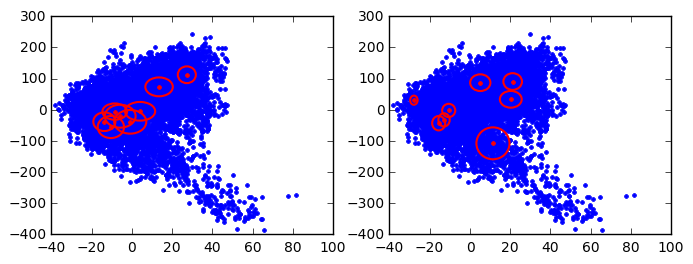
\includegraphics[width=\textwidth]{em_algorithm}
    \caption{Features 2 and 3 before (left) and after (right) the EM algorithm. The dashed blue lines are the 8 gaussians and the solid red lines the mixture.}
    \label{fig:em_algorithm}
\end{figure}

\subsubsection*{E-Step}

The expectation step consists of estimate the \emph{a posteriori} probabilities for each distribution $i$ and each feature vector $\dvec{x}_t$,

\begin{equation}
    \postprob{i}{\dvec{x}_t, \lambda} = \frac{w_i p_i(\dvec{x}_t)}{\sum_{k=1}^M w_k p_k(\dvec{x}_t)}.
    \label{eq:e-step-posterior}
\end{equation}

\subsubsection*{M-Step}

In the maximization step, the parameters are updated, and the algorithm guarantees that each new $\lambda^(j+1)$ represents the training data better than the previous ones. From \refbib{Reynolds}{reynolds.1995c}, the updates of $w_i$, $\dvec{\mu}_i$ and $\dvec{\Sigma}_i$ are given by the equations below.

\noindent\\\textbf{Weights:}

\begin{equation}
    \overline{w}_i = \frac{1}{T} \sum_{t=1}^T \postprob{i}{\dvec{x}_t, \lambda},
    \label{eq:m-step-weight}
\end{equation}

\noindent\\\textbf{Means:}

\begin{equation}
    \overline{\dvec{\mu}}_i = \frac{1}{T} \frac{\sum_{t=1}^T \postprob{i}{\dvec{x}_t, \lambda} \dvec{x}_t}{\sum_{t=1}^T \postprob{i}{\dvec{x}_t, \lambda}},
    \label{eq:m-step-means}
\end{equation}

\noindent\textbf{Variances:}

\begin{equation}
    \overline{\dvec{\sigma}}_i = \frac{1}{T} \frac{\sum_{t=1}^T \postprob{i}{\dvec{x}_t, \lambda} \dvec{x}_t^2}{\sum_{t=1}^T \postprob{i}{\dvec{x}_t, \lambda}} - \overline{\dvec{\mu}}_i^2.
    \label{eq:m-step-means}
\end{equation}
\\

This algorithm is used to train the GMMs described in sections \sectionref{speaker-identification} and \sectionref{speaker-verification} of \chapterref{speaker-recognition-system}. \figureref{em_algorithm} shows the mixture before and after the training.

\section{Universal Background Model}
\label{sec:ubm}

An Universal Background Model-Gaussian Mixture Model (UBM-GMM), shortened to UBM, is a GMM composed of features from all enrolled speakers. Its idea is to model a system as if speech signals were recorded by the same microphone with all speakers talking at once, i.e., a background of voices, a situation where it is impossible to understand the content of what each speaker is saying.

The training and evaluation of an UBM are the same for single speaker GMMs, with difference in the time taken (due to the number of speakers composing it). In this paper, there is two types of UBMs. In the first, the subpopulations of male and female speeches are combined and used to train a single, unisex UBM. In the second, each subpopulation is used to train its own model, and then both models are combined in one with twice the number of distributions.

\begin{figure}[ht]
    \centering
    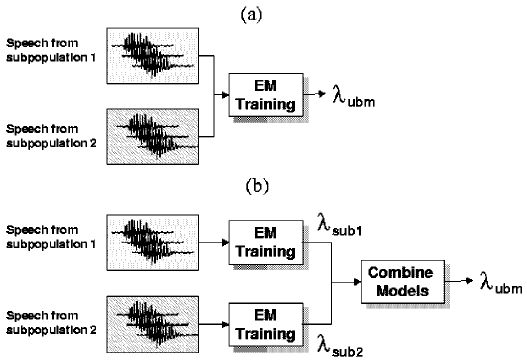
\includegraphics[width=0.7\textwidth]{ubm-diagram}
    \caption{Gender (a) independent and (b) dependent UBMs. \refbib{Reynolds, Quatieri \& Dunn}{reynolds.quatieri.dunn.2000}{}}
    \label{fig:ubm-diagram}
\end{figure}